\section{Neural network}

A neural network is a set of algorithms that attempts to recognize underlying relationships in a set of data using a process that mimics how the human brain works.
Neural network contains layers of interconnected nodes. 
Each node is known as a perceptron.

\subsection{Multilayer perceptron}

By adding one or more hidden layers, we can get around the drawbacks of linear models.
Stacking a lot of fully connected layers on top of one another is the simplest approach to accomplish this. 
Up until we produce outputs, each layer feeds into the layer above it. The first layers serve as our representation, and the top layer serves as our linear predictor. This design is frequently referred to as a \glsxtrfull{MLP}.

\begin{figure}[!h]
    \centering
    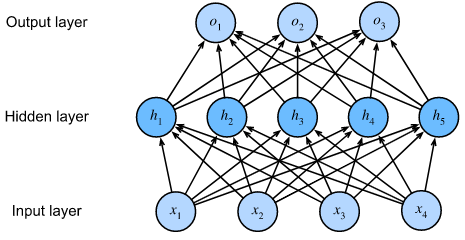
\includegraphics[width=0.7\textwidth]{figures/multilayer_perceptron.PNG}
    \caption{An MLP with a hidden layer of 5 hidden units \cite{zhang2021dive}}
    \label{multilayer_perceptron}
\end{figure}

This \glsxtrshort{MLP} has 4 inputs, 3 outputs, and 5 hidden units in its hidden layer.
Because the input layer does not require any computations, producing outputs with this network necessitates implementing computations for both the hidden and output layers; thus, the number of layers in this \glsxtrshort{MLP} is 2. 
It should be noted that both layers are fully connected. 
Every input influences every neuron in the hidden layer, and every neuron in the output layer influences every neuron in the hidden layer.

We denote by the matrix $X \in R^{n \times d}$ a minibatch of $n$ examples where each example has $d$ inputs (features). 
For a one-hidden-layer \glsxtrshort{MLP} whose hidden layer has $h$ hidden units, we denote by $H \in R^{n \times h}$ the outputs of the hidden layer, which are hidden representations. 
Since the hidden and output layers are both fully connected, we have hidden-layer weights $W^{(1)} \in R^{d \times h}$ and biases $b^{(1)} \in R^{1 \times h}$ and output-layer weights $W^{(2)} \in R^{h \times q}$ and biases $b^{(2)} \in R^{1 \times q}$. 
This allows us to calculate the outputs  of the one-hidden-layer MLP as follows:

\begin{equation}
\begin{aligned}
   H = X W^{(1)} + b^{(1)} \\
   O = H W^{(2)} + b^{(2)}
\end{aligned}
\end{equation}

To fully realize the potential of multilayer architectures, one more key component is required: a nonlinear activation function to be applied to each hidden unit after the affine transformation.
For instance, a popular choice is the ReLU (Rectified Linear Unit) activation function \cite{relu} $\sigma (x) = \max (0, x)$ operating on its arguments element-wise. 
The outputs of activation functions are called activations. 
In general, with activation functions in place, our \glsxtrshort{MLP} cannot be collapsed into a linear model.

\begin{equation}
\begin{aligned}
   H = \sigma (X W^{(1)} + b^{(1)}) \\
   O = H W^{(2)} + b^{(2)}
\end{aligned}
\end{equation}


\subsection{Training a neural network}

\textbf{Epoch}: one iteration where the model sees the whole training set to update its weights.

\textbf{Mini-batch gradient descent}: during the training phase, updating weights is usually not based on the whole training set at once due to computation complexities or one data point due to noise issues. 
Instead, the update step is done on mini-batches, where the number of data points in a batch is a hyperparameter (batch size) that we can tune.

\textbf{Loss function}: In order to quantify how a given model performs, the loss function $L$ is usually used to evaluate to what extent the actual outputs $y$ are correctly predicted by the model outputs $z$.

\textbf{Cross-entropy loss}: In the context of binary classification in neural networks, the cross-entropy loss $L(z,y)$ is commonly used and is defined as follows:
\begin{equation}
    L(z,y) = -[y \log (z) + (1-y) \log (1-z)]
\end{equation}

\textbf{Forward propagation}: The calculation and storage of intermediate variables (including outputs) for a neural network from the input layer to the output layer is referred to as forward propagation (or forward pass).

\textbf{Backpropagation}: The method of calculating the gradient of neural network parameters is known as backpropagation. In short, the method traverses the network in reverse order, from the output to the input layer, using calculus' chain rule. While calculating the gradient with respect to some parameters, the algorithm stores any intermediate variables (partial derivatives).

\textbf{Updating weights}: In a neural network, weights are updated as follows:

\begin{itemize}
    \item[] Step 1: Take a batch of training data and perform forward propagation (feedforward) to compute the loss.
    \item[] Step 2: Backpropagate the loss to get the gradient of the loss with respect to each weight
    \item[] Step 3: Use the gradients to update the weights of the network.
\end{itemize}

\begin{figure}[!h]
    \centering
    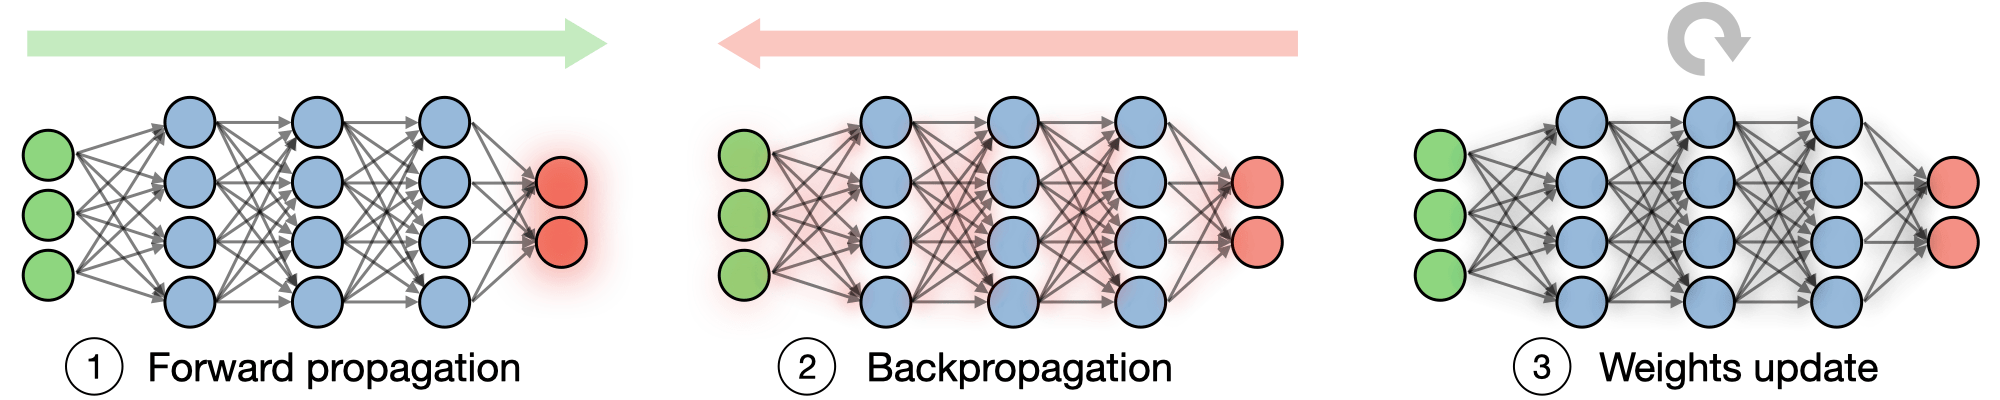
\includegraphics[width=1.0\textwidth]{figures/backpropagation.png}
    \caption{Updating weights in a neural network \cite{amidi2018deep}}
    \label{backpropagation}
\end{figure}


\subsection{Parameter tuning}

Weights initialization:
\begin{itemize}
    \item[] Xavier initialization \cite{xavier_init}: Rather than simply randomizing the weights, Xavier initialization allows for initial weights that take into account characteristics that are unique to the architecture. 
    Weights and inputs are centered at zero, while biases are initialized as zeros.
    \item[] Transfer learning: It is frequently useful to leverage pre-trained weights from massive datasets that took days/weeks to train and apply them to our use case. Figure \ref{transferlearning} shows some options for leveraging data, depending on how much we have:
\end{itemize}

%\begin{table}[!ht]
\centering
\begin{adjustbox}{width=0.9\columnwidth,center}
\begin{tabular}{|c|c|l|} 
\hline
\begin{tabular}[c]{@{}c@{}}\textbf{\textbf{Training }}\\\textbf{\textbf{size}}\end{tabular} & \textbf{\textbf{Illustration}} & \multicolumn{1}{c|}{\textbf{\textbf{Explanation}}}                                                                                                                                                                                                                                                               \\ 
\hline
\textcolor[rgb]{0.141,0.161,0.18}{Small}                                                    & \raisebox{-\totalheight}{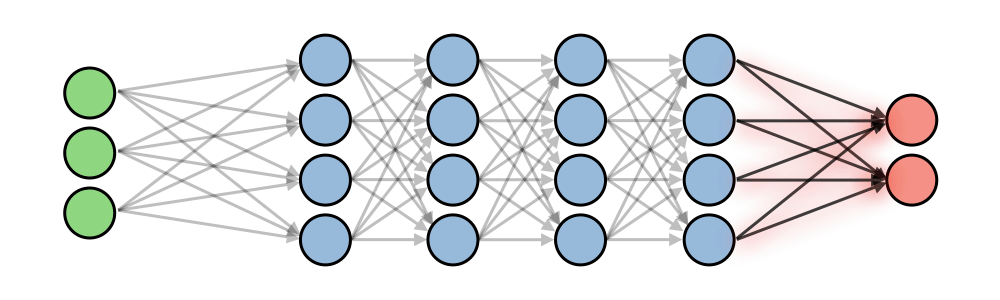
\includegraphics[width=0.7\textwidth, height=60mm]{figures/transfer-learning-small-ltr.png}}                       & \begin{tabular}[c]{@{}l@{}}\textcolor[rgb]{0.141,0.161,0.18}{Freezes all layers, }\\\textcolor[rgb]{0.141,0.161,0.18}{trains weights }\\\textcolor[rgb]{0.141,0.161,0.18}{on softmax}\end{tabular}                                                                                                               \\ 
\hline
\textcolor[rgb]{0.141,0.161,0.18}{Medium}                                                   & \raisebox{-\totalheight}{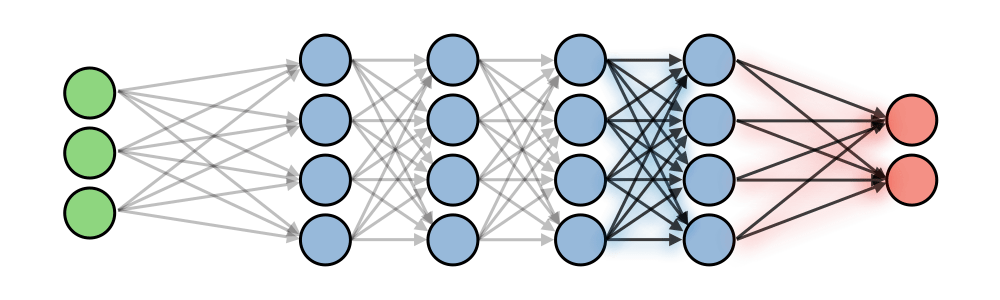
\includegraphics[width=0.7\textwidth, height=60mm]{figures/transfer-learning-medium-ltr.png}}                       & \begin{tabular}[c]{@{}l@{}}\textcolor[rgb]{0.141,0.161,0.18}{Freezes most }\\\textcolor[rgb]{0.141,0.161,0.18}{layers, trains weights }\\\textcolor[rgb]{0.141,0.161,0.18}{on last layers and }\\\textcolor[rgb]{0.141,0.161,0.18}{softmax}\end{tabular}                                                         \\ 
\hline
\textcolor[rgb]{0.141,0.161,0.18}{Large}                                                    & \raisebox{-\totalheight}{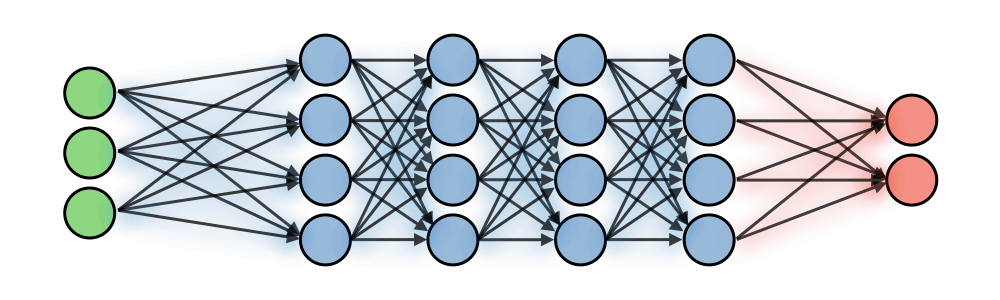
\includegraphics[width=0.7\textwidth, height=60mm]{figures/transfer-learning-large-ltr.png}}                       & \begin{tabular}[c]{@{}l@{}}\textcolor[rgb]{0.141,0.161,0.18}{Trains weights on }\\\textcolor[rgb]{0.141,0.161,0.18}{layers and softmax }\\\textcolor[rgb]{0.141,0.161,0.18}{by initializing }\\\textcolor[rgb]{0.141,0.161,0.18}{weights on }\\\textcolor[rgb]{0.141,0.161,0.18}{pre-trained ones}\end{tabular}  \\
\hline
\end{tabular}
\end{adjustbox}
\caption{Test}
\label{table:transfer_learning_strategy}
\end{table}
      
\begin{figure}[!h]
    \centering
    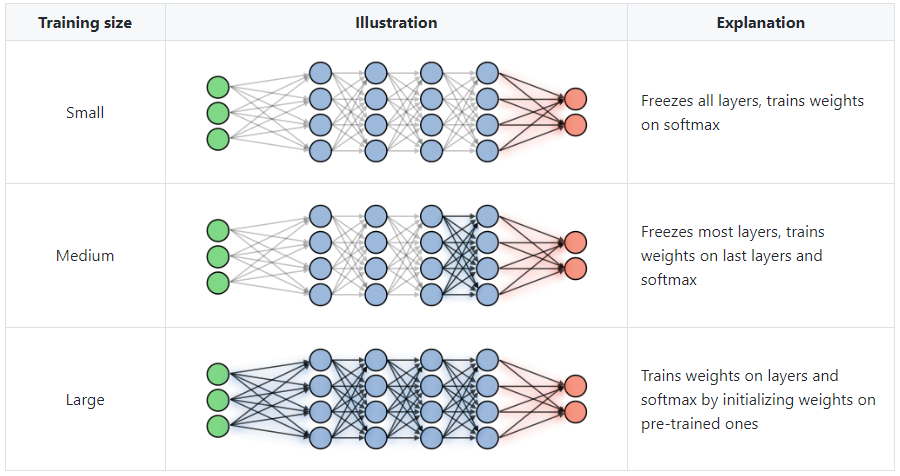
\includegraphics[width=1.0\textwidth]{figures/transferlearning.PNG}
    \caption{Transfer learning strategy \cite{amidi2018deep}}
    \label{transferlearning}
\end{figure}

Optimizing convergence:
\begin{itemize}
    \item[] Learning rate: indicates how quickly the weights are updated. 
    It can be fixed or changed adaptively. 
    The most popular method at the moment is Adam \cite{kingma2015adam}, which is a method that adapts the learning rate.
    \item[] Adaptive learning rates: Allowing the learning rate to vary when training a model can help to reduce training time while also improving the numerical optimal solution. While the Adam optimizer is the most commonly used technique, the following in figure \ref{adaptiveLR} are also useful:
\end{itemize}

\begin{figure}[!h]
    \centering
    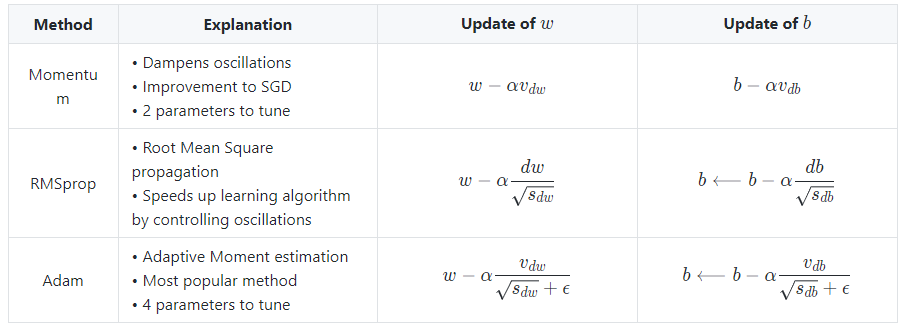
\includegraphics[width=0.95\textwidth]{figures/adaptiveLR.PNG}
    \caption{Adaptive learning rates methods \cite{amidi2018deep}}
    \label{adaptiveLR}
\end{figure}

Regularization:

\begin{itemize}
    \item[] Dropout \cite{dropout}: to avoid overfitting the training data by removing neurons with probability $p > 0$. 
    It forces the model to avoid relying too heavily on specific sets of features.
    \item[] Weight regularization: Regularization techniques are typically used on the model weights to ensure that the weights are not too large and that the model is not overfitting the training set.
    \item[] Early stopping: to halt training as soon as the validation loss reaches a plateau or begins to rise.
    \item[] SpecAugment \cite{park2019specaugment}: Rather than augmenting the input audio waveform, SpecAugment applies an augmentation policy directly to the audio spectrogram (i.e., an image representation of the waveform).
    The spectrogram is altered by warping it in time, masking blocks of consecutive frequency channels, and masking blocks of utterances in time.
    These augmentations are chosen to help the network to be robust against deformations in the time direction, partial loss of frequency information and partial loss of small segments of speech of the input.
\end{itemize}


\subsection{Convolutional Neural Network}

Architecture of a traditional \glsxtrfull{CNN} is generally composed of the following layers:
\begin{itemize}
    \item[] Convolution layer (CONV): This layer employs filters that perform convolution operations while scanning the input $I$ in terms of its dimensions. 
    The filter size $F$ and stride $S$ are two of its hyperparameters. 
    The resulting output $O$ is referred to as a feature map or an activation map.
    \item[] Pooling layer (POOL): a downsampling operation used after a convolution layer to achieve spatial invariance. 
    Max and average pooling, in particular, are types of pooling that take the maximum and average value, respectively.
    \item[] Fully connected layer (FC): works with a flattened input, with each input connected to all neurons. 
    FC layers, when present, are typically found near the end of \glsxtrshort{CNN} architectures and can be used to optimize objectives such as class scores.
\end{itemize}


\subsection{Recurrent Neural Network}

\glsxtrfull{RNN} is a deep learning model that captures the dynamics of sequences through recurrent connections, which can be viewed as node cycles in a network (connections between nodes can create a cycle).
\glsxtrshort{RNN}s are unrolled across time steps (or sequence steps) using the same underlying parameters at each step. 
While standard connections are used synchronously to propagate activations from one layer to the next at the same time step, recurrent connections are dynamic, passing information across adjacent time steps.
As illustrated in Figure \ref{rnn}, \glsxtrshort{RNN}s are feedforward neural networks in which the parameters of each layer (both conventional and recurrent) are shared across time steps.

\begin{figure}[!h]
    \centering
    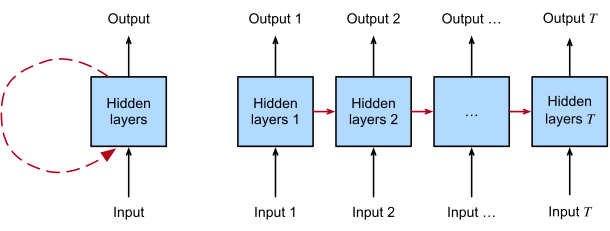
\includegraphics[width=1.0\textwidth]{figures/unfolded-rnn.png}
    \caption{Recurrent connections are depicted on the left as cyclic edges. The RNN is unfolded over time steps on the right. Recurrent edges are computed synchronously, while conventional connections span adjacent time steps. \cite{zhang2021dive}}
    \label{rnn}
\end{figure}


\subsection{Bidirectional Long Short-Term Memory}

The most popular designs include mechanisms to mitigate \glsxtrshort{RNN}s' infamous numerical instability, as exemplified by vanishing and exploding gradients.
We present the key concepts underlying the most successful \glsxtrshort{RNN} architectures for sequence, which are based on two papers published in 1997.

\glsxtrfull{LSTM} \cite{lstm1997} is the first paper to introduce the memory cell, a unit of computation that replaces traditional nodes in a network's hidden layer.
With these memory cells, networks can overcome training difficulties encountered by previous recurrent networks. 
To avoid the vanishing gradient problem, the memory cell keeps values in each memory cell's internal state cascading along a recurrent edge with weight 1 across many successive time steps. 
A set of multiplicative gates assists the network in determining which inputs to allow into the memory state and when the memory state's content should influence the model's output.
Given memory cell $c_t$, input gate $i_t$, forget gate $f_t$, output gate $o_t$ associated with weight matrices $W_j$, $U_j$ and weight vector $b_j$ where $j \in \{i, f, o, c\}$, \glsxtrshort{LSTM} is described as:

\begin{equation}
\begin{aligned}
   i_{t} &= \operatorname{sigmoid}_{g}(W_{i}x_{t} + U_{i}h_{t-1} + b_{i}) \\
   f_{t} &= \operatorname{sigmoid}_{g}(W_{f}x_{t} + U_{f}h_{t-1} + b_{f}) \\
   o_{t} &= \operatorname{sigmoid}_{g}(W_{o}x_{t} + U_{o}h_{t-1} + b_{o}) \\
   c_{t} &= f_{t} \odot c_{t-1} + i_{t} \odot \operatorname{sigmoid}_{c}(W_{c}x_{t} + U_{c}h_{t-1} + b_{c}) \\
   h_{t} &= o_{t} \odot \operatorname{sigmoid}_{h}(c_{t}) 
\end{aligned}
\end{equation}

The second paper, Bidirectional \glsxtrfull{RNN} \cite{brnn1997}, describes an architecture that uses information from both the future (subsequent time steps) and the past (preceding time steps) to determine the output at any point in the sequence. 
This is in contrast to previous networks, in which only previous input could influence output. 
Bidirectional \glsxtrshort{RNN}s have become a mainstay in audio sequence labeling tasks, among many others. 
Fortunately, the two innovations are not mutually exclusive and have been successfully combined for phoneme classification and handwriting recognition.


\subsection{Transformer}

The Transformer employs the encoder-decoder architecture, as shown in the left and right halves of Figure \ref{transformer_blocks}, with stacked self-attention and point-wise, fully connected layers for both the encoder and decoder.

\begin{figure}[!h]
    \centering
    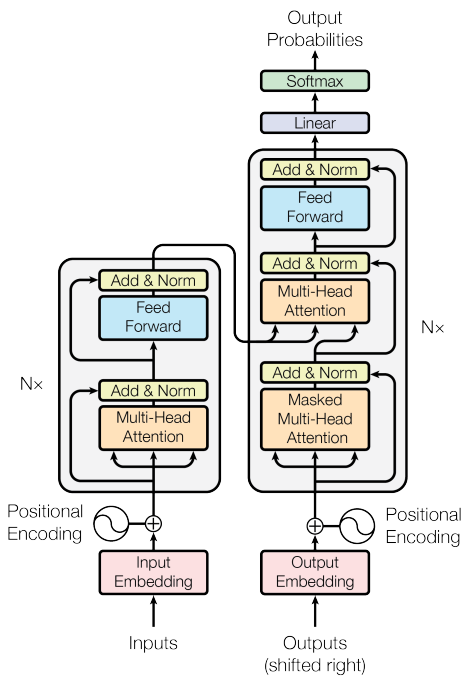
\includegraphics[width=0.5\textwidth]{figures/transformer_blocks.PNG}
    \caption{The Transformer model architecture \cite{Transformer}}
    \label{transformer_blocks}
\end{figure}

The encoder is built up from N identical layers. 
Each layer is divided into two sub-layers. 
The first is a multi-head self-attention mechanism, and the second is a simple, fully connected feed-forward network that is positionally connected. 
Following layer normalization \cite{layer_normalization}, a residual connection \cite{DeepResidualLearning} is used around each of the two sub-layers.

\textbf{Attention}: A query and a set of key-value pairs are mapped to an output by an attention function, where the query, keys, values, and output are all vectors. 
The output is computed as a weighted sum of the values, with the weight assigned to each value determined by the query's compatibility function with the corresponding key.

\textbf{Scaled Dot-Product Attention}: The input consists of
queries and keys of dimension $d_{k}$, and values of dimension $d_{v}$.
The query's dot products are computed with all keys, divided by $\sqrt d_{k}$, and a softmax function is applied to get the weights on the values.
In practice, we compute the attention function on a set of queries at the same time, which we pack into a matrix $Q$. 
The keys and values are also packed into matrices $K$ and $V$. 
We compute the output matrix as follows:

\begin{equation}
    \operatorname{Attention}(Q, K, V ) = \operatorname{softmax}(\frac{QK^{T}}{\sqrt d_{k}}) V
\end{equation}

\textbf{Multi-Head Attention}: Instead of performing a single attention function with $d_{model}$-dimensional keys, values and queries, we perform the attention function in parallel on each of the projected versions of queries, keys, and values, yielding $d_{v}$-dimensional output values.
These are concatenated and projected again, yielding the final values:

\begin{equation}
    \operatorname{MultiHead}(Q, K, V ) = \operatorname{Concat}(\mathrm{head}_{1}, ..., \mathrm{head}_{h})W^{O}
\end{equation}

where: $\mathrm{head}_{i} = \operatorname{Attention}(QW_{i}^{Q}, KW_{i}^{K}, VW_{i}^{V})$ 

and the projections are parameter matrices $W_{i}^{Q} \in R^{d_{\mathrm{model}} \times d_{k}}$, $W_{i}^{K} \in R^{d_{\mathrm{model}} \times d_{k}}$, $W_{i}^{V} \in R^{d_{\mathrm{model}} \times d_{v}}$ and $W^{O} \in R^{hd_{v} \times d_{\mathrm{model}}}$,

$h$ is the number of attention heads.
